\setcounter{page}{1}
\pagenumbering{arabic}

\chapter{Introduction}
\label{Introduction}
\thispagestyle{empty}

\begin{quotation}
{\footnotesize
\noindent{\emph{``\greek{L'egein t`a progen'omena, gin'wskein t`a pare'onta, prol'egein t`a >es'omena:
			 melet~an ta~uta. >Aske~in per`i t`a nos'hmata d'uo, >wfele~in <`h m`h bl'aptein.
			 >H t'eqnh di`a tri~wn, t`o n'oshma ka`i <o  nos'ewn ka`i <o >ihtr'oc:
			 <o >ihtr'oc <uphr'ethc t~hc t'eqnhc, <upenantio~usjai t~w| nos'hmati t`on nos'eonta met`a to~u >ihtro~u. }\\
			 (The physician must be able to tell the antecedents, know the present, and foretell the future:
			 must mediate these things, and have two special objects in view with regard to disease, to do good or to do no harm.
			 The art consists in three things: the disease, the patient, and the physician.
			 The physician is the servant of the art, and the patient must combat the disease along with the physician.)''}
}
\begin{flushright}
\greek{<Ippokr'athc}(Hippocrates, Epid. 1.2.11)
\end{flushright}
}
\end{quotation}

\vspace{2cm}

%\noindent L'introduzione deve essere atomica, quindi non deve contenere n\`e sottosezioni n\`e paragrafi n\`e altro. Il titolo, il sommario e l'introduzione devono sembrare delle scatole cinesi, nel senso che lette in quest'ordine devono progressivamente svelare informazioni sul contenuto per incatenare l'attenzione del lettore e indurlo a leggere l'opera fino in fondo. L'introduzione deve essere tripartita, non graficamente ma logicamente:


%\section{Inquadramento generale}
%La prima parte contiene una frase che spiega l'area generale dove si svolge il lavoro; una che spiega la sottoarea pi\`u specifica dove si svolge il lavoro e la terza, che dovrebbe cominciare con le seguenti parole ``lo scopo della tesi \`e \dots'', illustra l'obbiettivo del lavoro. Poi vi devono essere una o due frasi che contengano una breve spiegazione di cosa e come \`e stato fatto, delle attivit\`a  sperimentali, dei risultati ottenuti con una valutazione e degli sviluppi futuri. La prima parte deve essere circa una facciata e mezza o due

Cancer, or in medical terms \textit{malignant neoplasm}, identifies a wide range of diseases, all of which involve unregulated cell growth \cite{rubin1998genetic}.
While normal cells follow a normal process of growth, division, and death, cancer cells begin to form when this transformation breaks down, as they continue to
expand and divide. This leads to a mass of abnormal cells that grows out of control.
Healthy tissue can be invaded by cancer cells; it can harm the body when the
abnormal cells start to form masses of tissue, known as tumors, which
can interfere with the body's system and function.\\

\clearpage

There are about 200 known types of cancer\footnote{\url{http://www.cancerresearchuk.org/cancer-help/about-cancer/cancer-
questions/how-many-different-types-of-cancer-are-there}} and breast cancer is the most frequent type of cancer among women
worldwide \cite{sariego2010breast}, as also reported by \Gls{IARC}\footnote{\url{http://globocan.iarc.fr/factsheets/populations/factsheet.asp?uno=900#WOMEN}}, with about 22.9\% of
incidence and 13.7\% of mortality \cite{breastCancerIncidence}.\\
Prognosis and survival rates for breast cancer vary greatly depending on the cancer type, stage, treatment, and geographical location of the patient.\\
Early detection of cancer stage plays an important role in selecting the best treatments and reducing cancer mortality.
The current procedure for breast cancer grading is manually performed by pathologists, as
breast tissue samples of patients are taken and examined under microscopes.\\

\vspace{0.5cm}

Pathologists grade the tissue samples based on the deviation of the cell structures
from normal tissues. A pathologist may have to examine hundreds of slides daily \cite{histopat01}, which is a subjective and time consuming process.\\
Histopathological images (images of biopsy samples) are now available in high resolution digital format, which can be further
processed to extract useful structural information.\\
With the growth of computer and image technology, medical imaging has greatly influenced
medical field. As the quality of medical imaging affects diagnosis, the medical
image processing has become an interesting research topic, not only for the ability to store, retrieve and handling a large amount of data, but rather for 
automating the analysis process \cite{medImagingReview01}.\\

\vspace{0.5cm}

A cell that divides itself into two daughter cells with the same chromosomes undergoes a process of \textit{mitosis}
(see Figure \ref{ch1:fig1})\footnote{image taken from \url{http://en.wikipedia.org/wiki/Mitosis}}.

\begin{figure}[!htbf]
 \centering
  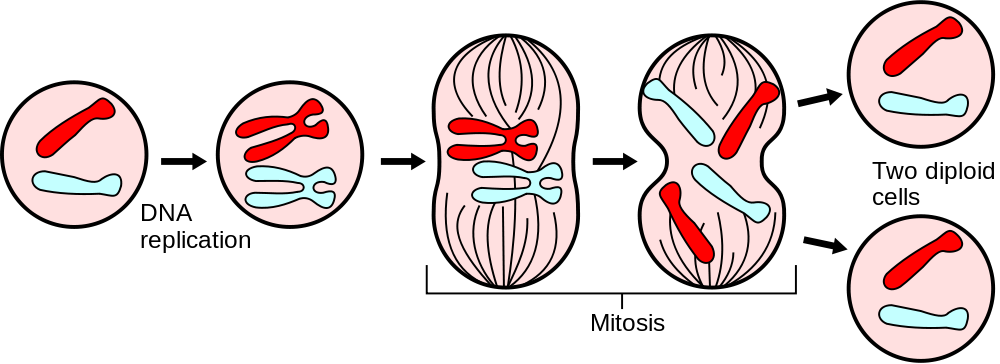
\includegraphics[width=0.92\textwidth]{./images/Major_events_in_mitosis.png}
  \caption{Mitosis of a cell}
  \label{ch1:fig1}
\end{figure}

\vspace{0.5cm}


The scoring of mitotic figures is an integrated part of the various systems for grading of invasive breast cancer with most rigorous criteria \cite{breastCancerGrading01}.
For this reason, the automatic detection and counting of mitotic figures in breast cancer tissue is an attractive and challenging research
topic \cite{Mitosis01}.\\
An example of histological images for mitosis detection is given in Figure \ref{ch1:fig2}\footnote{image taken from \url{ttp://www.breastpathology.info}}.

\begin{figure}[!hbt]
  \centering
    \subfigure{
      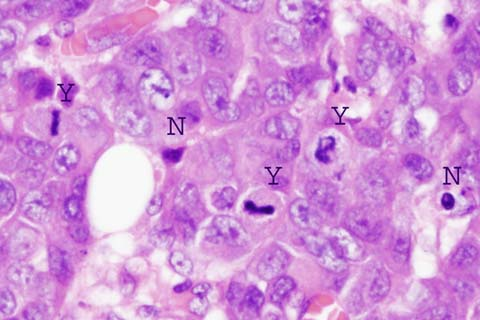
\includegraphics[width=0.47\textwidth]{./images/bcg0.jpg}
      %\label{ch1:fig2:a}
    }
    \hspace{0.1mm}
    \subfigure{
      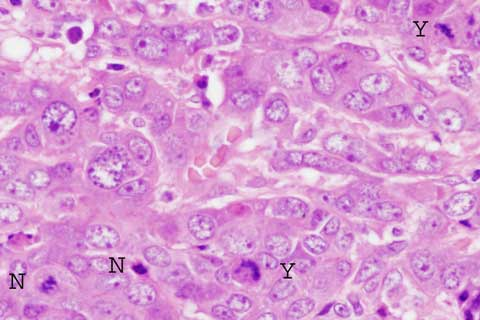
\includegraphics[width=0.47\textwidth]{./images/bcg2.jpg}
      %\label{ch1:fig2:b}
    }\\
    \vspace{0.1mm}
    \subfigure{
      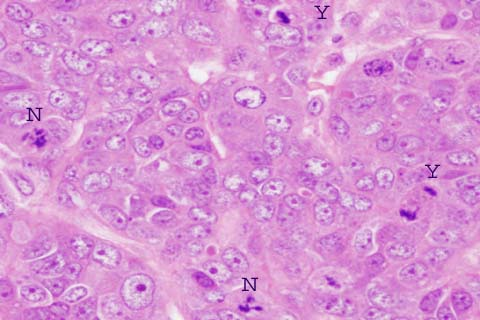
\includegraphics[width=0.47\textwidth]{./images/bcg3.jpg}
      %\label{ch1:fig2:c}
    }
    \hspace{0.1mm}
    \subfigure{
      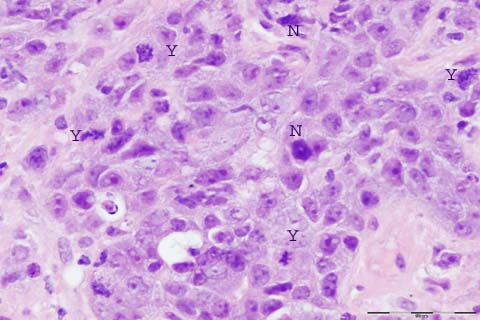
\includegraphics[width=0.47\textwidth]{./images/bcg5.jpg}
      %\label{ch1:fig2:d}
    }
    \caption[Histological images with labeled mitoses and non-mitoses]{Histological images with labeled mitoses (\texttt{Y}) and non-mitoses (\texttt{N})}
    \label{ch1:fig2}
\end{figure}


The automatic detection process lays its groundwork in the fields of Computer Vision and Machine Learning\cite{mitosisBreastCancerImagingAlgorithmsTHESIS}.
Mitotic cells must be found and identified on a histological image. This issue can be faced as a
detection problem, to find interesting portions of a histological image, and a supervised learning problem, where a classifier
is given a set of labeled samples (mitoses and non-mitoses) from which it must gain some information to classify unseen samples.\\

% \clearpage

\noindent Various aspects influence the performances of such automatic processes, which can be summarized into:

\begin{itemize}
 \item the size and the quality of the dataset,
 \item the ability of the classifier to gain information and to generalize.
\end{itemize}

The quality of the dataset is related the idea of data validation form a clinical point of view. Mitosis detection is known to be
a difficult problem, and several studies have found that pathologists' agreement on the mitotic grade is fairly modest, with strong biases \cite{mitoticRecognition03Agreement}.
This aspect have an impact when using data to train a a computerized system for mitosis detection.\\
Conversely, once a dataset and the associated ground truth is accepted, it is the classifier that has to be able to gain information on labeled samples and
use this information to perform sufficiently well on new (unseen) data.

\vspace{0.5cm}

From the application point of view, both aspects (dataset and classifier performance) are important to build a reliable automatic mitosis detection system:
the most relevant issue is whether such algorithms perform similarly (or better) than experts who routinely solve the same task.

Instead, in this work we put ourselves in the perspective of the machine learning algorithm designer. Within this context, comparing a
mitosis detection algorithm with an expert pathologist does not provide
much useful information, because they are not competing on a fair basis. In fact, during
his formation and previous activity, a pathologist had access to an amount of training information (in form of criteria, guidelines and labeled examples) which is
most probably extremely larger than every algorithm's training set. The question that arises is: if the algorithm
underperforms, is it because it is not powerful enough, or because it has not enough data to learn?
The former case means that the effort should be focused on improving the algorithm ability, the latter implies that effort should be instead focused on gathering larger labeled datasets.
We aim to answer this question in the context of mitosis detection in breast
cancer histological images using a public dataset.

\vspace{0.5cm}

In our work we focused on the classification problem, extracting labeled samples from images of a public dataset annotated by an expert pathologist.
We then built some classifiers based on such images and implemented a testing website to collect classifications by different users.
We compared the performances of our classifiers with the ones obtained by algorithms participating to the 
\textit{ICPR 2012 Mitosis Detection Contest}\footnote{\url{http://ipal.cnrs.fr/ICPR2012/?q=node/1}}(performance measured on the same dataset) and with performances of humans facing the same problem.\\
Our test subjects were given no guidelines, and were required to
learn a classification function solely from the provided training set.
This kind of setting can not be recreated when benchmarking humans for other famous instances of visual pattern recognition problems (such as
face detection, object recognition, and handwriting understanding). One of such
benchmarks \cite{ML_traffic} focused on the task of classifying traffic sign images, which is a
significantly easier problem than mitosis classification; algorithms were given a
very large training set (25000 images) and the best algorithm outperformed the best
individual (among 8) with an accuracy of 99.46\% vs 99.22\%.
These results are consistent with the ones that we report in this work, based on 7 algorithms and 45 test subjects, compared to 2 different classifiers developed ad hoc.




\vspace{0.5cm}

%\section{Inquadramento generale}
%La prima parte contiene una frase che spiega l'area generale dove si svolge il lavoro; una che spiega la sottoarea pi\`u specifica dove si svolge il lavoro e la terza, che dovrebbe cominciare con le seguenti parole ``lo scopo della tesi \`e \dots'', illustra l'obbiettivo del lavoro. Poi vi devono essere una o due frasi che contengano una breve spiegazione di cosa e come \`e stato fatto, delle attivit\`a  sperimentali, dei risultati ottenuti con una valutazione e degli sviluppi futuri. La prima parte deve essere circa una facciata e mezza o due

%\section{Breve descrizione del lavoro}
%La seconda parte deve essere una esplosione della prima e deve quindi mostrare in maniera pi\`u esplicita l'area dove si svolge il lavoro, le fonti bibliografiche pi\`u importanti su cui si fonda il lavoro in maniera sintetica (una pagina) evidenziando i lavori in letteratura che presentano attinenza con il lavoro affrontato in modo da mostrare da dove e perch\'e \`e sorta la tematica di studio. Poi si mostrano esplicitamente le realizzazioni, le direttive future di ricerca, quali sono i problemi aperti e quali quelli affrontati e si ripete lo scopo della tesi. Questa parte deve essere piena (ma non grondante come la sezione due) di citazioni bibliografiche e deve essere lunga circa 4 facciate.

\noindent The dissertation presents the following structure:

\begin{itemize}
 \item In Chapter \ref{chapter2} we review the state of the art in the main fields of research in which our 
 work is included, such as: mitosis detection for breast cancer grading, applications of computer vision techniques
 in biomedical imaging, and machine learning methods for biomedical classification.
 \item In Chapter \ref{chapter3} we define the problem of mitosis counting, in terms of detection and classification.
 We also describe some implementations of mitosis detection algorithm and define the most important measures of performance for classification task.
 \item In Chapter \ref{chapter4} we describe the dataset on which all our work is based and define the framework for the classification algorithms that
 we implemented. We outline the main components needed to carry out a classification task: dataset manipulation, features selection and extraction, 
 classification and analysis of the performances.
 \item In Chapter \ref{chapter5} we describe the testing website developed to collect users' classifications and performance.
 \item In Chapter \ref{chapter6} we describe all the experimental results deriving from automatic classification, human classification and we compare
 the results.
 \item Chapter \ref{chapter7} is dedicated to conclusions and evaluations on possible future research directions.
\end{itemize}

One appendix is included in this work: Appendix \ref{appendixD} shows some of the image samples used for our classification tasks.

% \begin{itemize}
%  \item Appendix \ref{appendixA} describes the process of mitosis in cells.
%  \item Appendix \ref{appendixB} reports the main components of the code written for automatic classification.
%  \item Appendix \ref{appendixC} describes the software structure of the testing website.
%  \item Appendix \ref{appendixD} shows some of the image samples used for our classification tasks.
% \end{itemize}



%\section{Struttura della tesi}
%La terza parte contiene la descrizione della struttura della tesi ed \`e organizzata nel modo seguente.
%``La tesi \`e strutturata nel modo seguente.

%Nella sezione due si mostra \dots

%Nella sez. tre si illustra \dots

%Nella sez. quattro si descrive \dots

%Nelle conclusioni si riassumono gli scopi, le valutazioni di questi e le prospettive future \dots

%Nell'appendice A si riporta \dots (Dopo ogni sezione o appendice ci vuole un punto).''

%I titoli delle sezioni da 2 a M-1 sono indicativi, ma bisogna cercare di mantenere un significato equipollente nel caso si vogliano cambiare. Queste sezioni possono contenere eventuali sottosezioni.
 

%\Gls{naiive} people don't know about alternative \gls{computer} operating systems: \glspl{Linux}, BSDs and GNU/Hurd.